\documentclass[a4paper, 12pt]{article}

\usepackage[utf8x]{inputenc}
\usepackage[T2A]{fontenc}
\usepackage[english, russian]{babel}
\usepackage{mathtools}
\usepackage{newtxmath}
\usepackage[left=0.3cm,right=1cm,top=1cm, bottom=2cm, bindingoffset=1cm]{geometry}
\usepackage{enumerate}
\usepackage{enumitem}
\usepackage[usenames]{color}
\usepackage{graphicx}
\usepackage{listings}

\DeclareRobustCommand{\divby}{
  \mathrel{\text{\vbox{\baselineskip.65ex\lineskiplimit0pt\hbox{.}\hbox{.}\hbox{.}}}}%
}
\title{\textbf{Поиск контура объединения прямоугольников}}
\author{Ахмедов Садрудин}
\date{}



\begin{document}
\maketitle


\section*{Алгоритм поиска контура}
Алгоритм анализирует множество прямоугольников с сторонами, параллельными осям координат, и строит их объединённый контур. Основные шаги:

\begin{itemize}
\item Входные данные: координаты левого нижнего и правого верхнего углов прямоугольников $(x_1,y_1,x_2,y_2)$
\item Используется алгоритм сканирующей прямой (sweep line)
\item Определяются все критические точки по оси $X$
\item Для каждой вертикальной полосы вычисляется пересечение прямоугольников
\item Формируется список рёбер итогового контура
\end{itemize}

\section*{Клиент-серверная архитектура}
\begin{itemize}
\item \textbf{Сервер} (на C++):
\begin{itemize}
\item Принимает координаты прямоугольников
\item Обрабатывает алгоритмом
\item Возвращает точки контура
\end{itemize}
\item \textbf{Клиент} (на C++):
\begin{itemize}
\item Отправляет данные на сервер
\item Получает и визуализирует результат
\end{itemize}

\item Особенности:
\begin{itemize}
\item Использует fork() для обработки множества клиентов
\item TCP-соединение с бинарной передачей данных
\item Оптимизированная обработка больших наборов данных
\end{itemize}
\end{itemize}

\section*{Результаты работы}
Пример визуализации контура:

\begin{figure}[h]
\centering
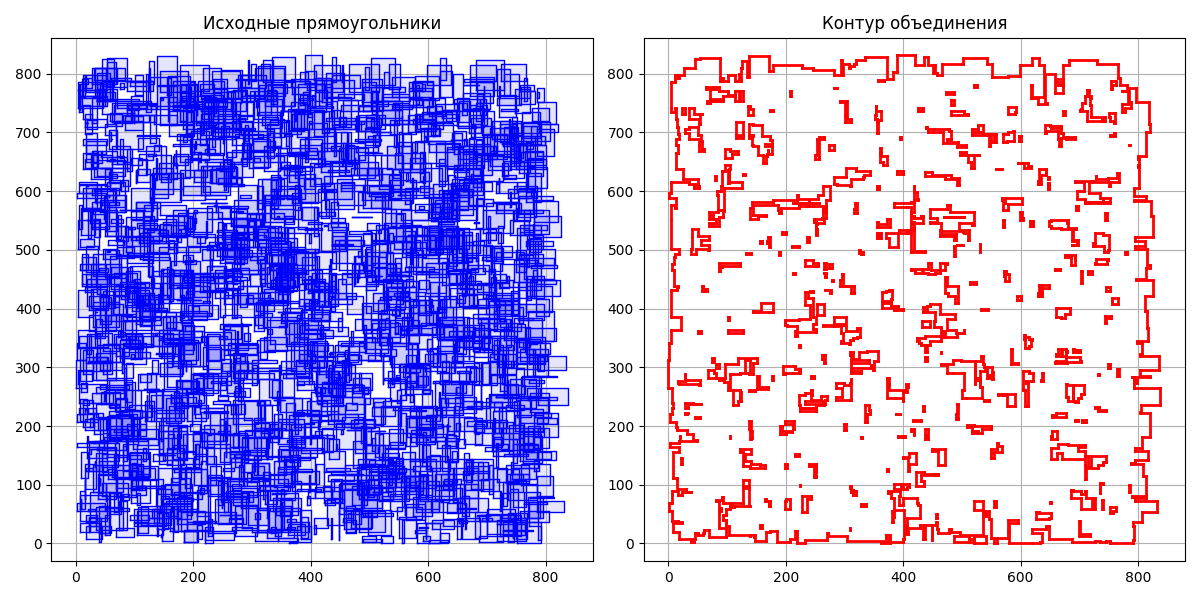
\includegraphics[width=0.8\textwidth]{contour_example.png}
\caption{Пример объединения прямоугольников}
\end{figure}

\section*{Вывод}
Проект успешно реализует:
\begin{itemize}
\item Эффективный алгоритм геометрических вычислений
\item Стабильную клиент-серверную коммуникацию
\item Масштабируемую обработку данных
\end{itemize}

\end{document}